% ================= 1 MOTIVATION =================
\section{Motivation}

\begin{frame}{Engine design trend}
  \centering
  \vspace{-0.55cm}{Turbofan engines are getting larger as they are more efficient}\par
  \vspace{.35cm}
  \begin{columns}[c]
    \column{.47\textwidth}\centering
    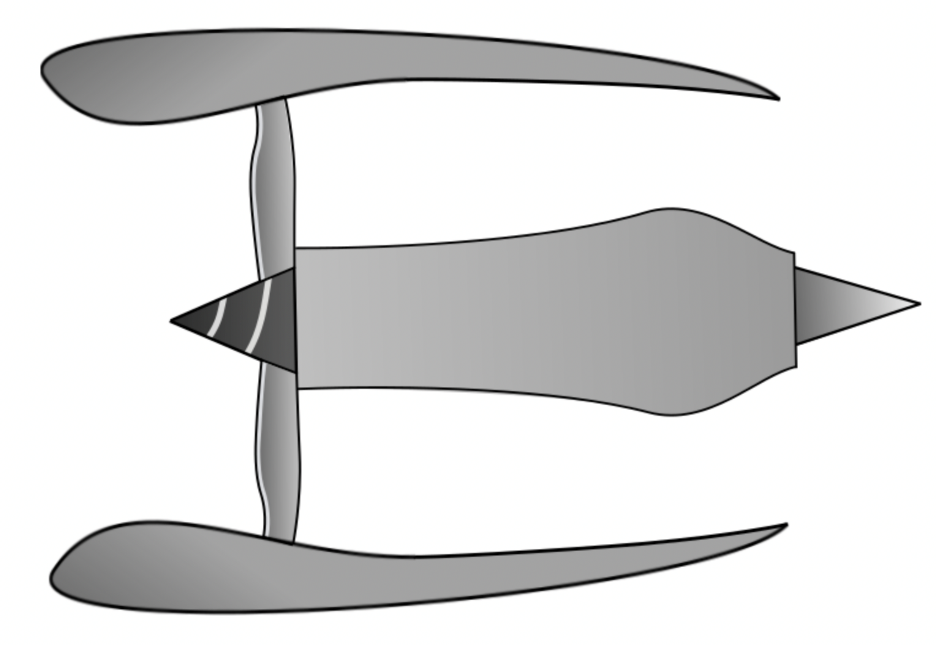
\includegraphics[width=5.5cm,keepaspectratio]{figures/old_engine.png}
    \column{.47\textwidth}\centering
    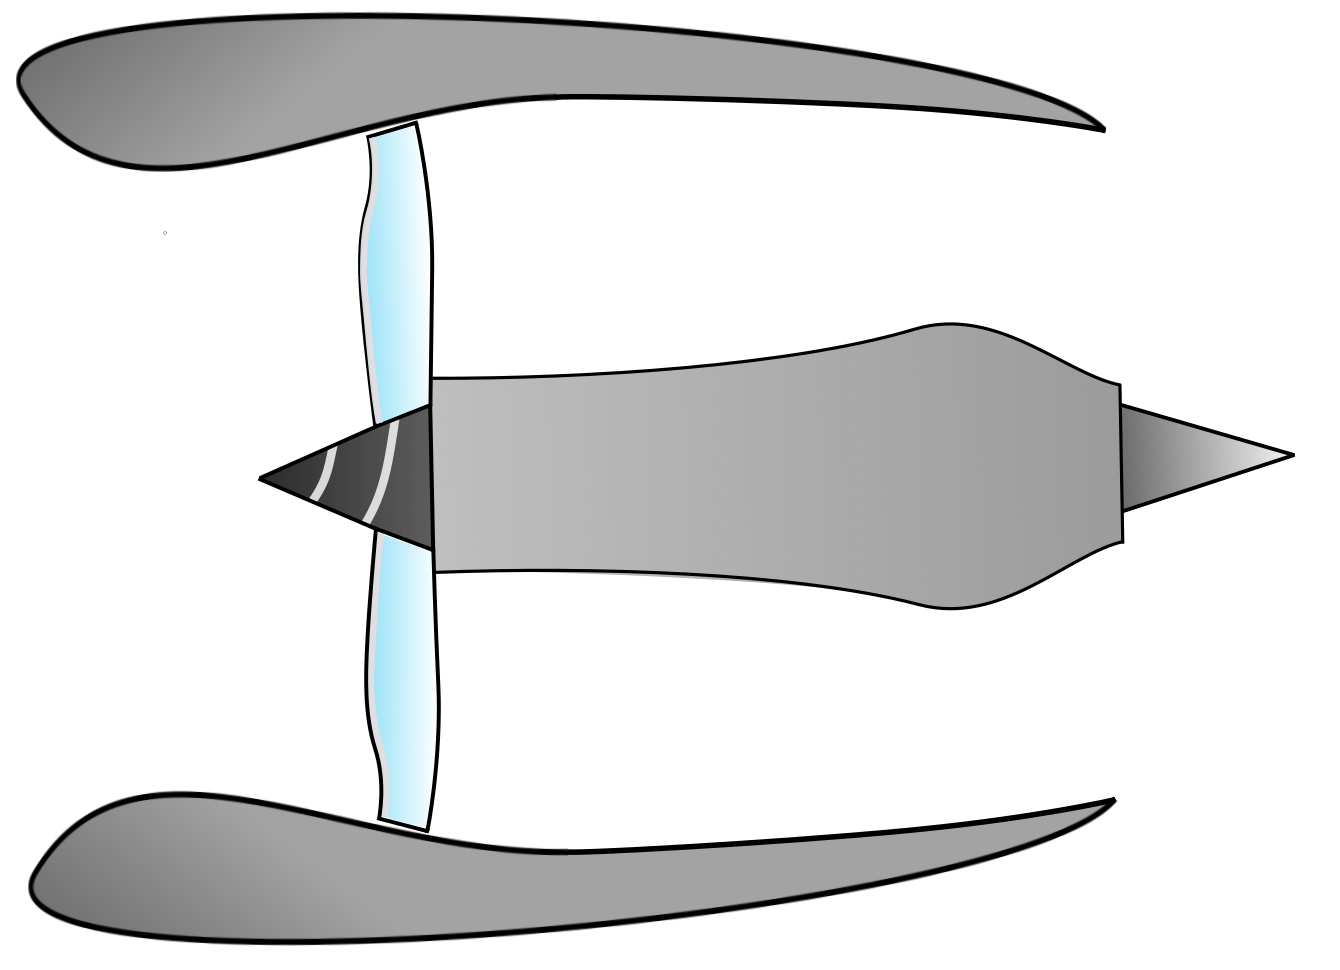
\includegraphics[width=6.5cm,height=4.6cm,keepaspectratio]{figures/new_engine.png}\par
  \end{columns}
  \vspace{.50cm}
  \begin{columns}[T]
    \column{0.47\textwidth}\centering
    \footnotesize{OLD: smaller fan, lower bypass ratio}
    \column{0.47\textwidth}\centering
    \footnotesize\textcolor{teal}{NEW: Larger fan, higher bypass ratio}
  \end{columns}
  \vspace{.35cm}
  \only<2>{\textbf{\textcolor{red}{Problem: larger nacelles have more drag}}}
\end{frame}

\begin{frame}{How do we reduce nacelle drag?}
  \only<1>{\centering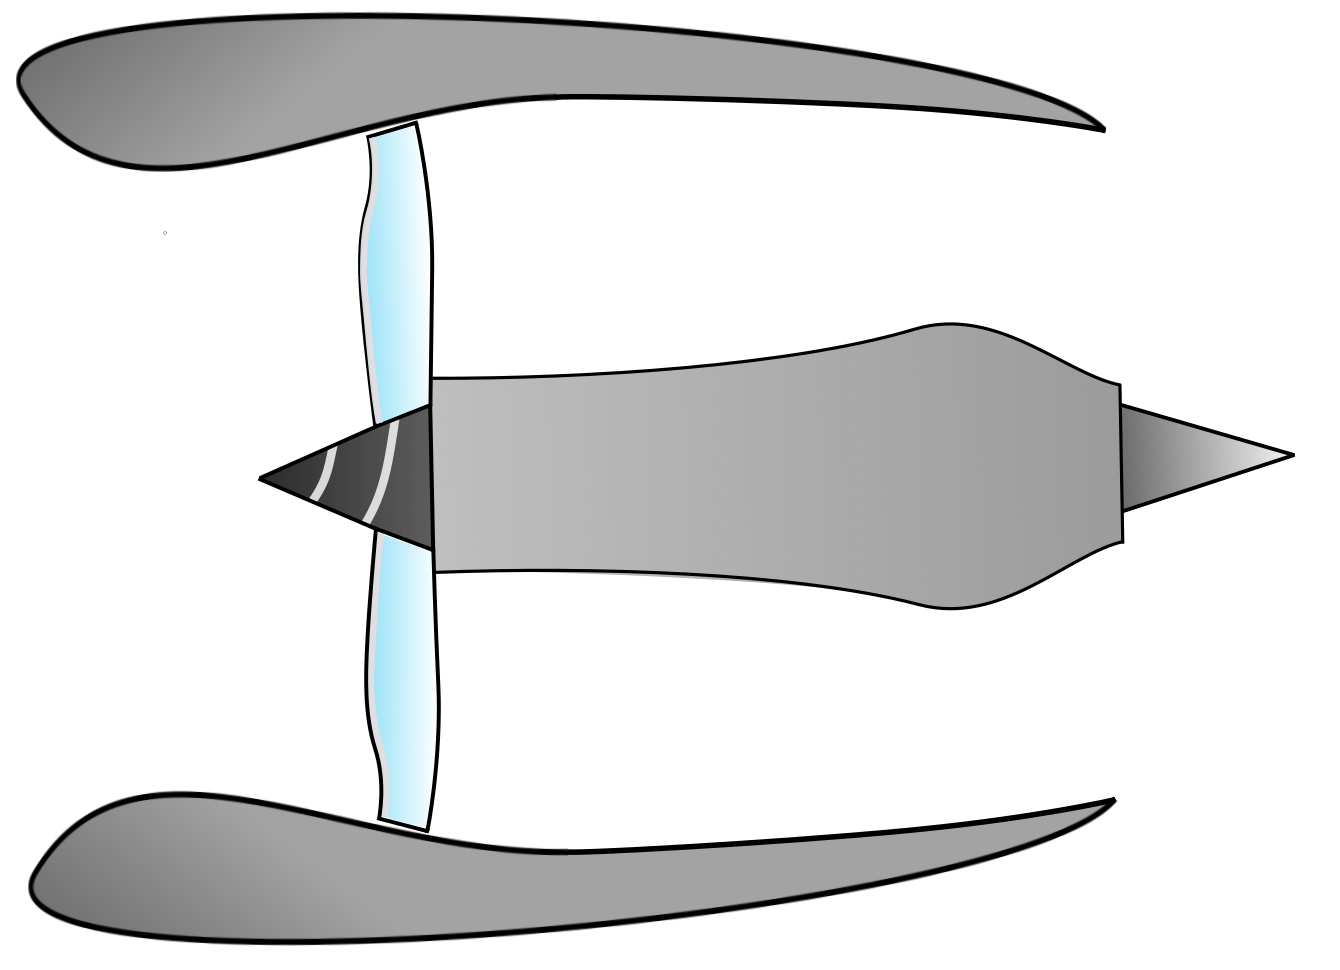
\includegraphics[width=7.0cm,height=5.3cm,keepaspectratio]{figures/new_engine.png}}
  \only<2>{
  \begin{columns}[c]
    \column{.52\textwidth}\centering
    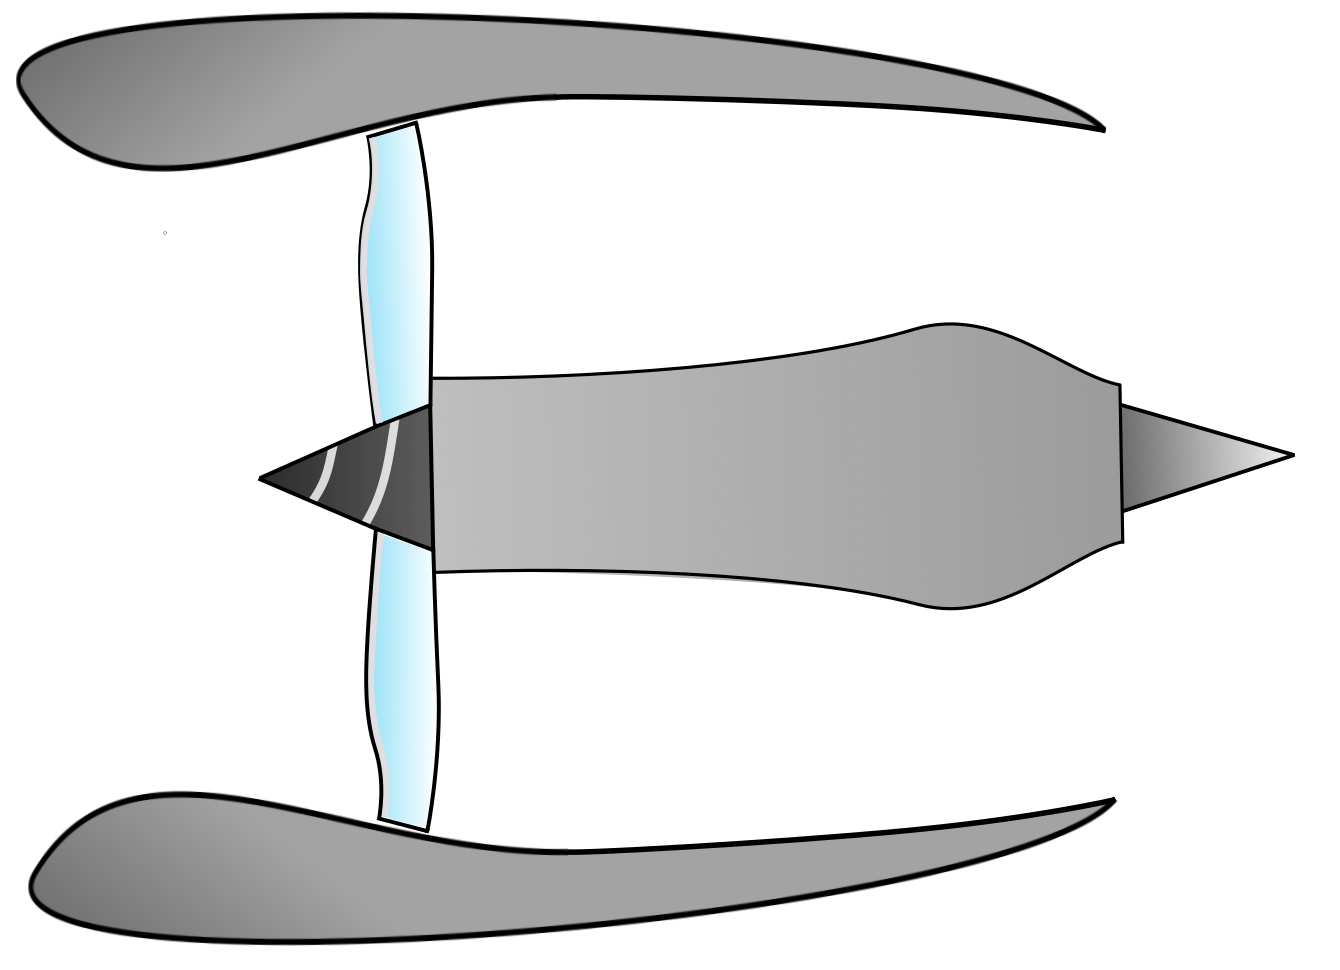
\includegraphics[width=7.0cm,height=5.3cm,keepaspectratio]{figures/new_engine.png}
    \column{.42\textwidth}
  \end{columns}
  }
  \only<3->{
    \begin{columns}[c]
      \column{.52\textwidth}\centering
      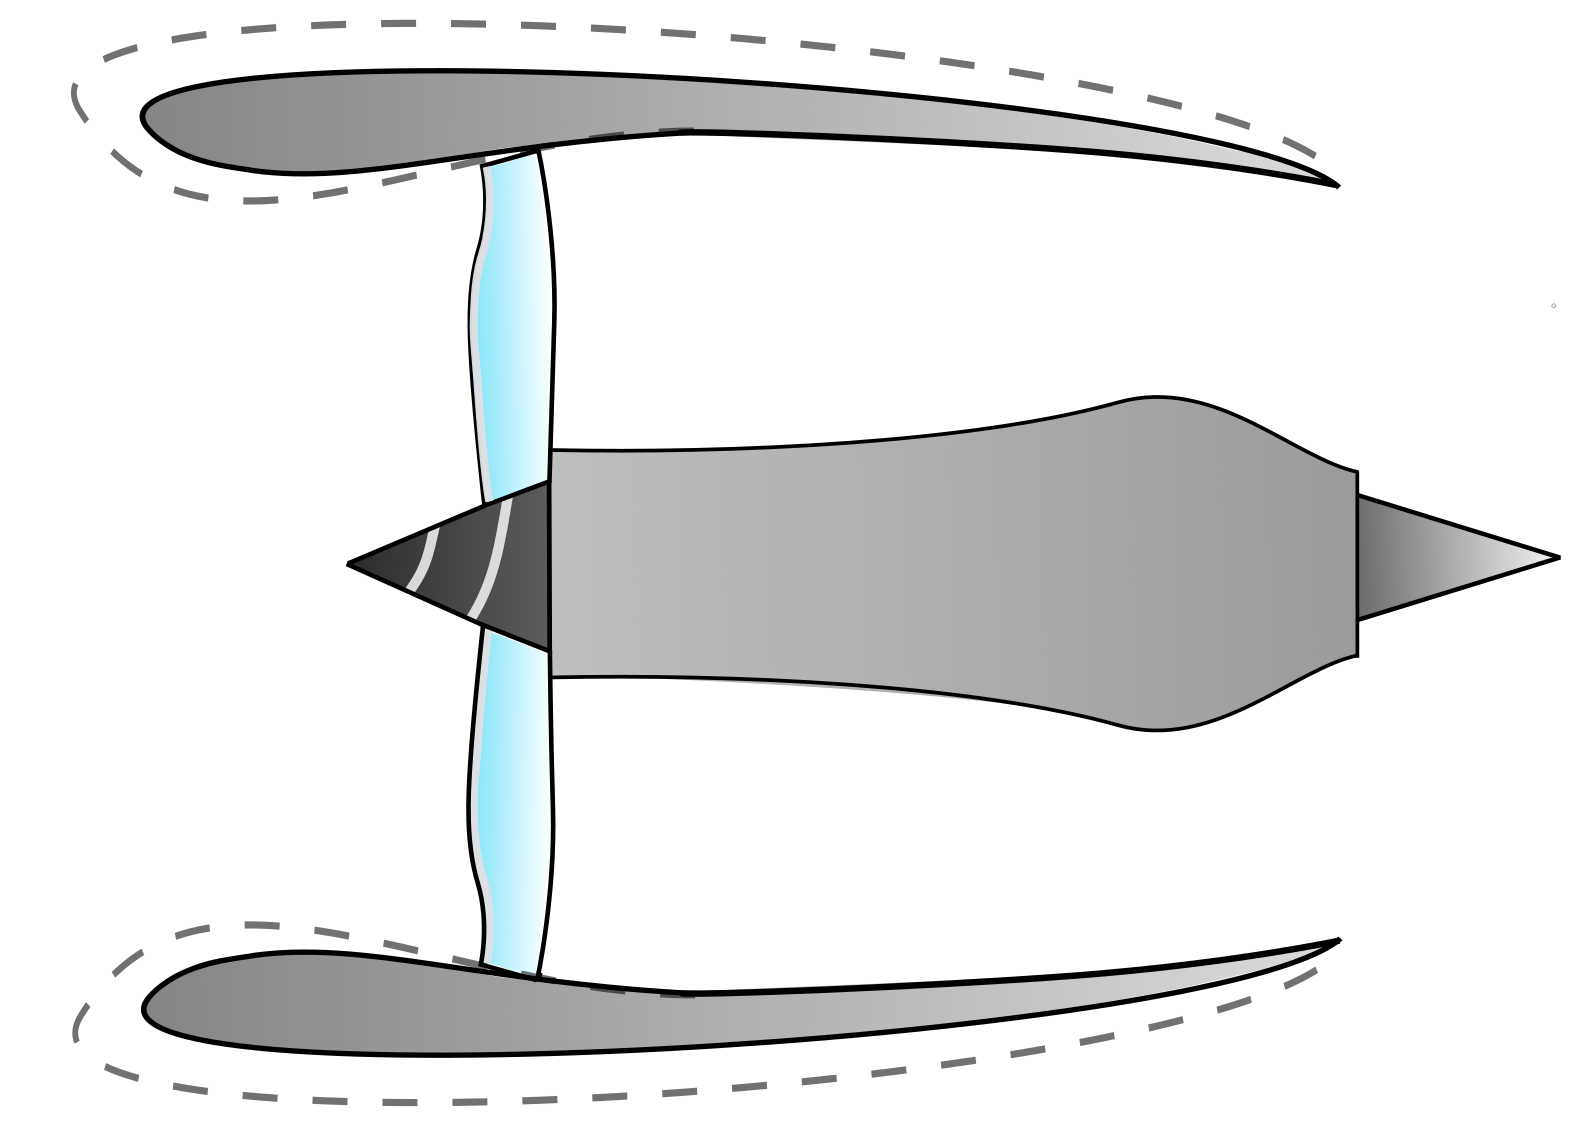
\includegraphics[width=7.0cm,height=5.3cm,keepaspectratio]{figures/engine_shorter_nacelle.png}

      \column{.45\textwidth}
      \begin{itemize}\setlength\itemsep{1em}
        \item Use a shorter, sharper nacelle.
        \item Increase the curvature of the lip.
      \end{itemize}
      \uncover<4>{
      \vspace{1em}
      \hspace{0.8em}
      \card{amber}{Challenge}{What happens during off-design conditions?}}
    \end{columns}
  }
\end{frame}

\begin{frame}{Crosswind creates an off-design threat}
  \begin{columns}[c]
    \column{.62\textwidth}\centering
    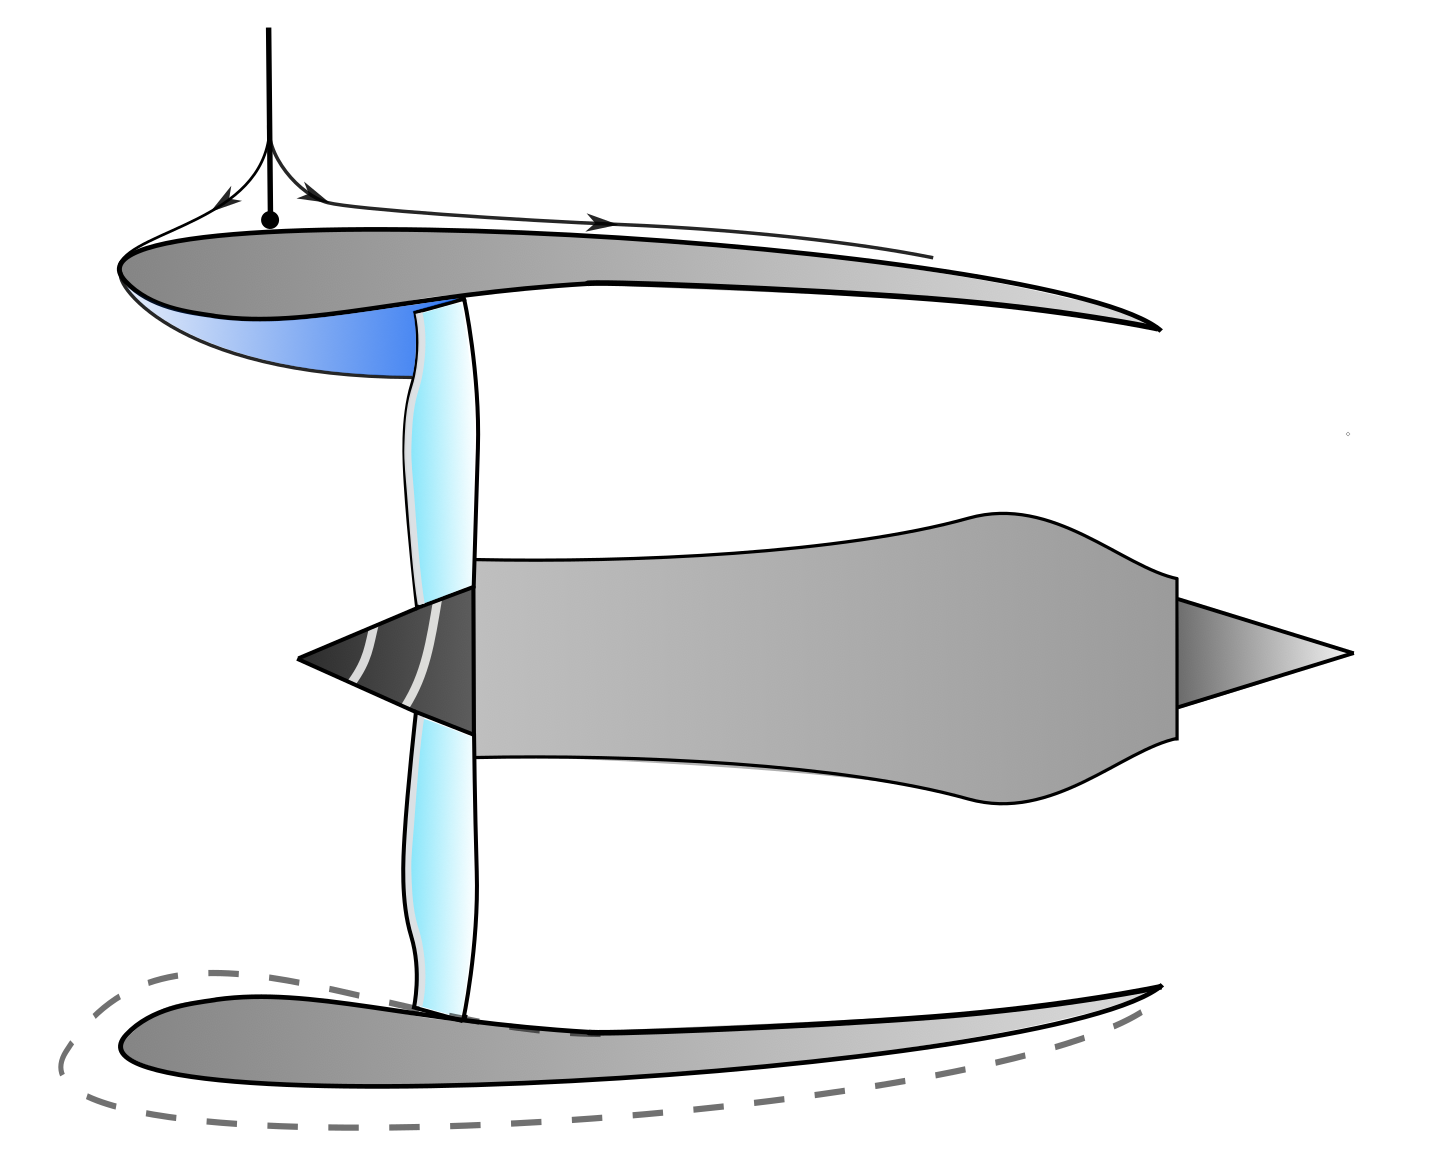
\includegraphics[width=7.2cm,height=5.2cm,keepaspectratio]{figures/engine_crosswind.png}

    \column{.50\textwidth}
    \begin{itemize}\setlength\itemsep{1em}
      \setlength{\itemindent}{-1em}
      \setlength{\leftmargin}{-3em}
      \item Smaller radius of curvature at the lip
      \uncover<2->{\item \textbf{Higher risk of separation of the flow}}
      \uncover<3->{\item Stronger acceleration of the flow}
      \uncover<4->{\item Flow can reach supersonic speeds}
      \uncover<5->{\item \textbf{More frequent SBL interations and \\ \hspace{-1.2em} separation}}
    \end{itemize}
  \end{columns}
\end{frame}

\begin{frame}{Possible windward-lip flowfields}
  \centering
  \begin{columns}[T]
    \column{.235\textwidth}\centering
    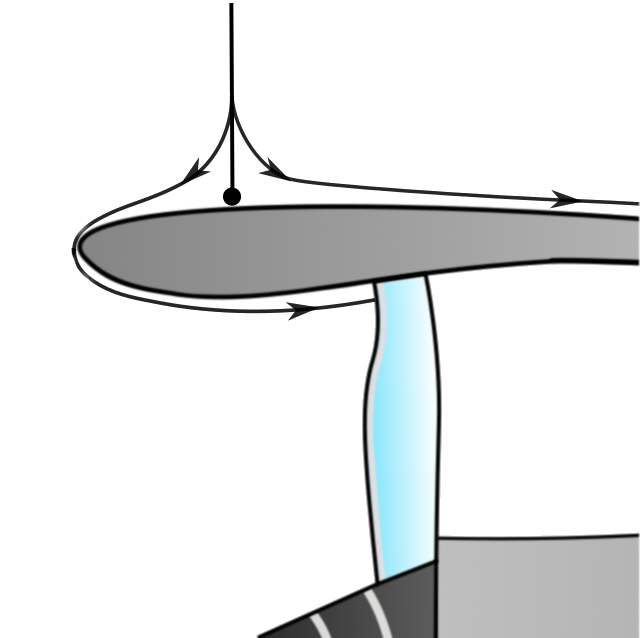
\includegraphics[width=3.15cm,height=3.65cm,keepaspectratio]{figures/subsonic_attached.png}\par\vspace{2pt}
    \textbf{Subsonic}\par\small Attached boundary layer

    \column{.235\textwidth}\centering
    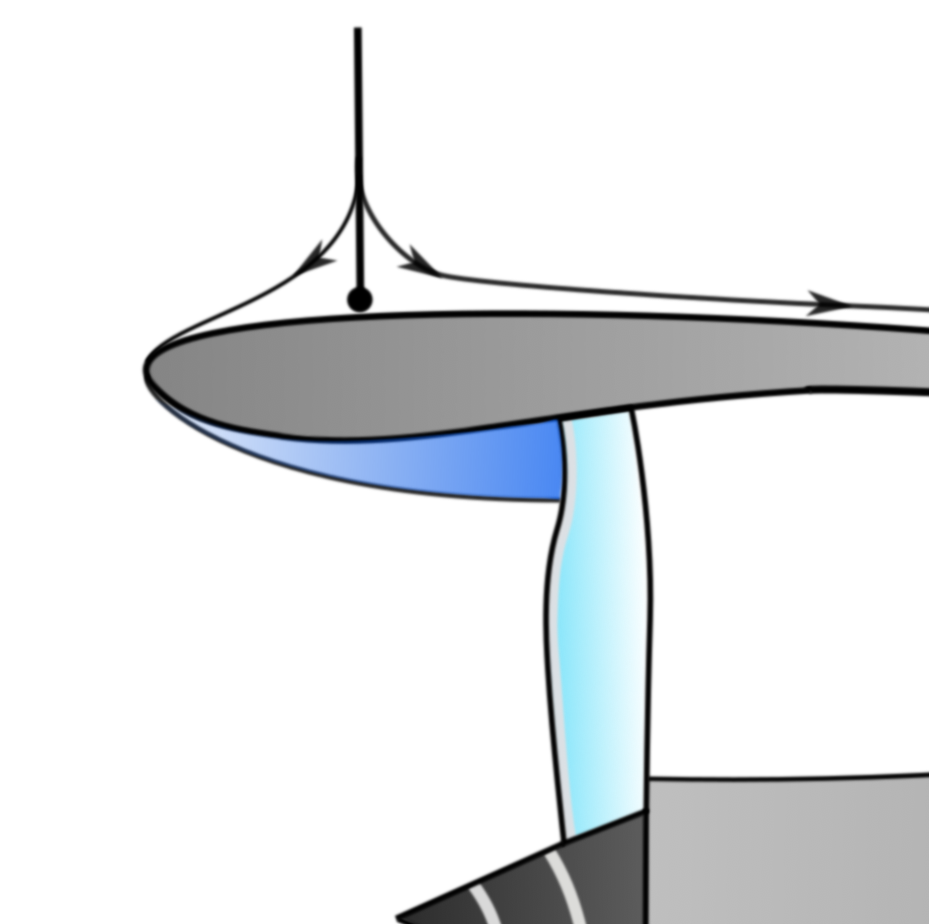
\includegraphics[width=3.15cm,height=3.65cm,keepaspectratio]{figures/subsonic_separated.png}\par\vspace{2pt}
    \textbf{Subsonic}\par\small\alert{Diffusive boundary layer separation}

    \column{.235\textwidth}\centering
    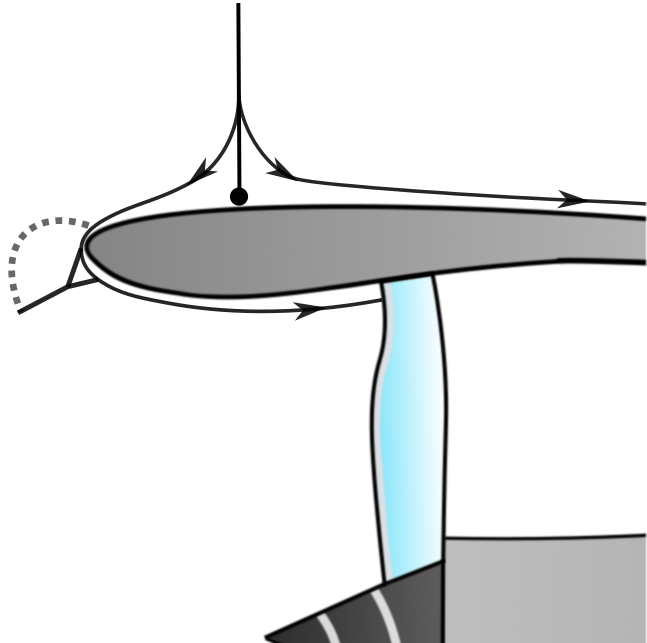
\includegraphics[width=3.15cm,height=3.65cm,keepaspectratio]{figures/supersonic_attached.png}\par\vspace{2pt}
    \textbf{Supersonic}\par\small Attached boundary layer

    \column{.235\textwidth}\centering
    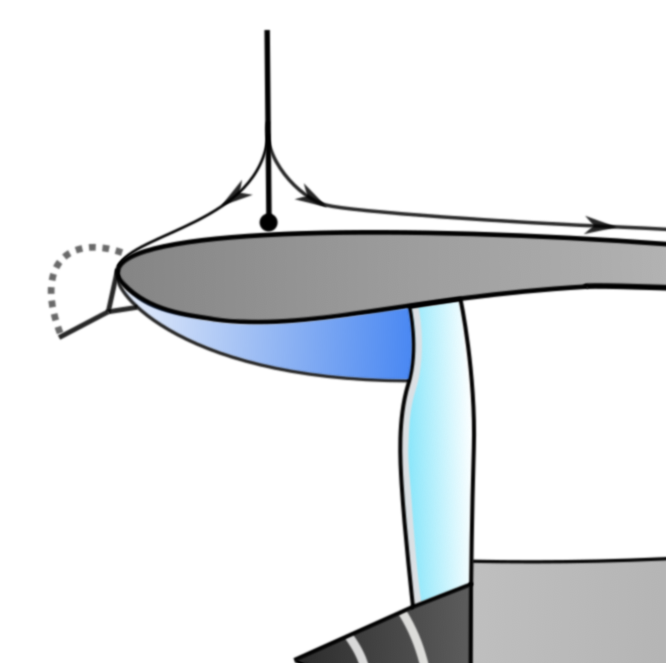
\includegraphics[width=3.15cm,height=3.65cm,keepaspectratio]{figures/supersonic_separated.png}\par\vspace{2pt}
    \textbf{Supersonic}\par\small\alert{Shock-induced separation}
  \end{columns}
  \vspace{.18cm}
  % \textbf{The research question:} How do these states couple together.....
\end{frame}

\begin{frame}{How we replicate the engine intake in the wind tunnel}
  \centering
    \only<1>{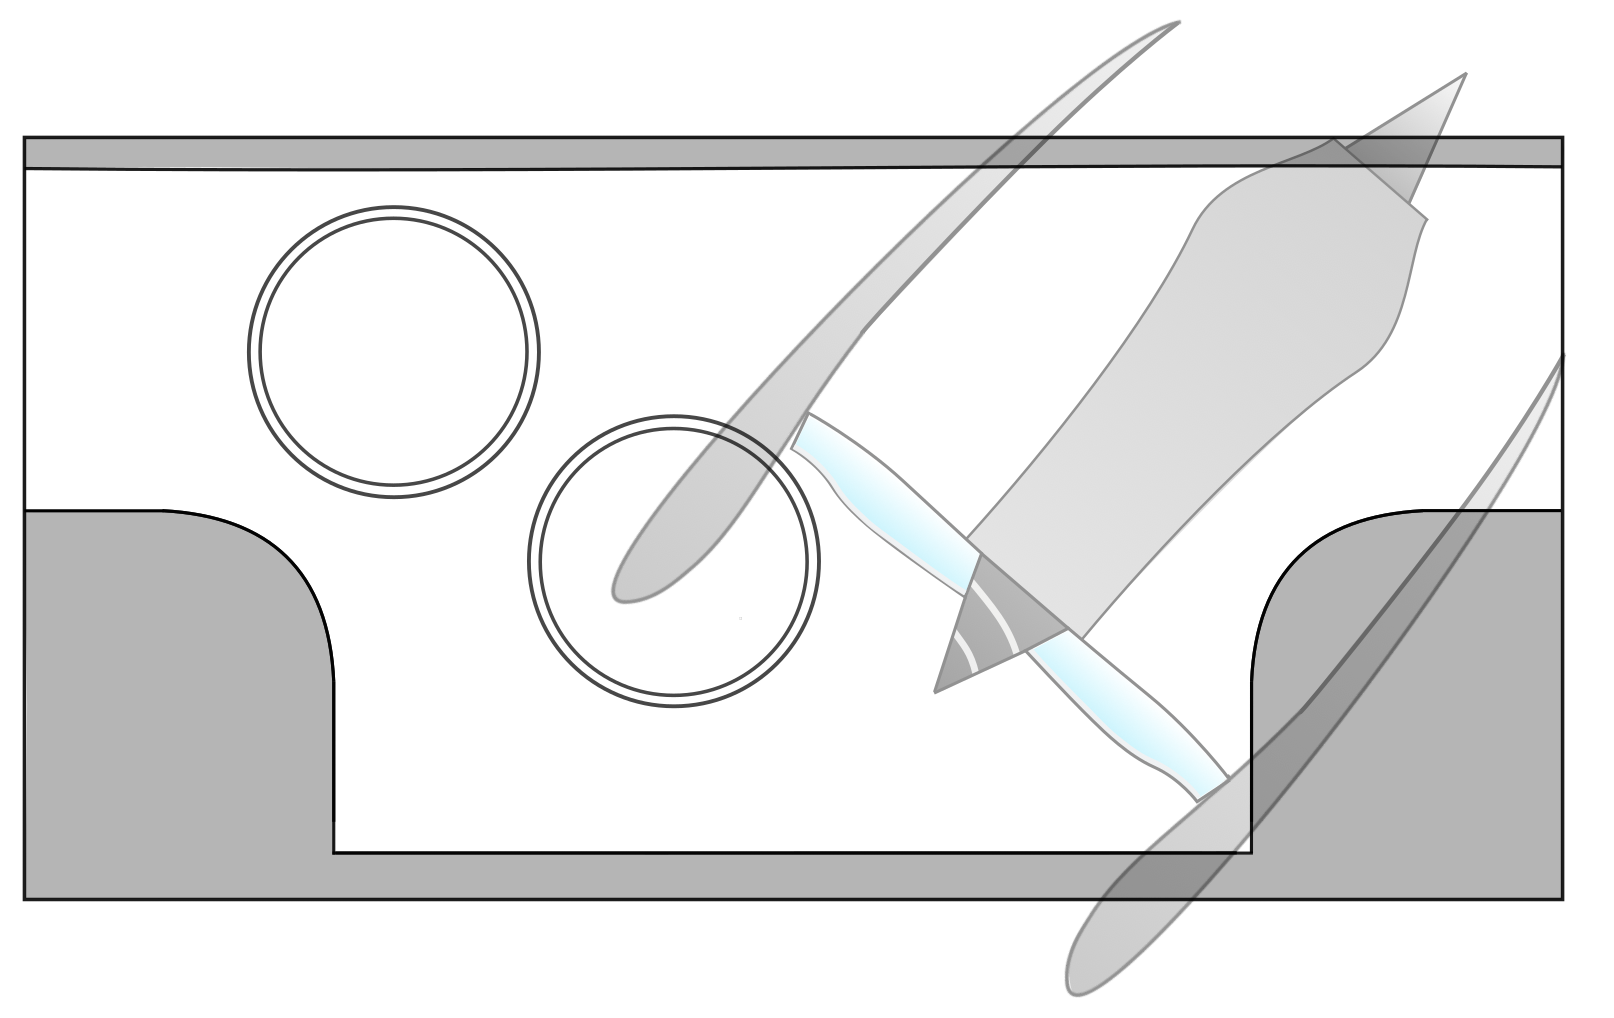
\includegraphics[width=10.1cm,keepaspectratio]{figures/engine_in_windtunnel.png}}
    \only<2>{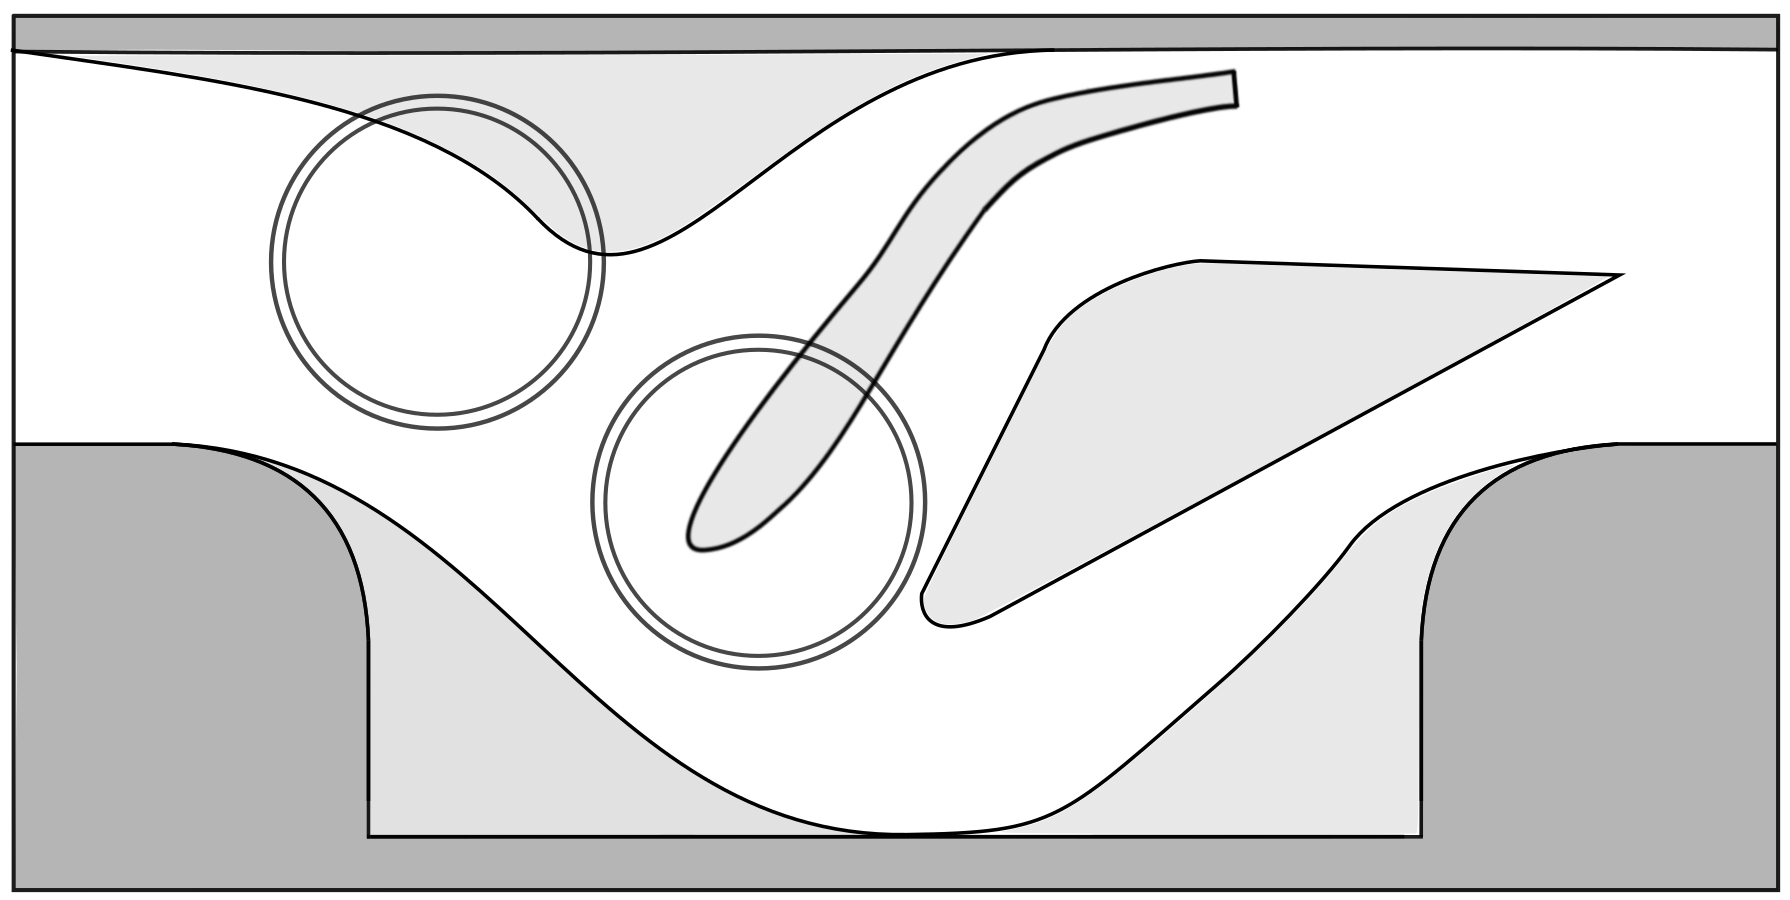
\includegraphics[width=10.1cm,keepaspectratio]{figures/wind_tunnel.png}}
    \only<3->{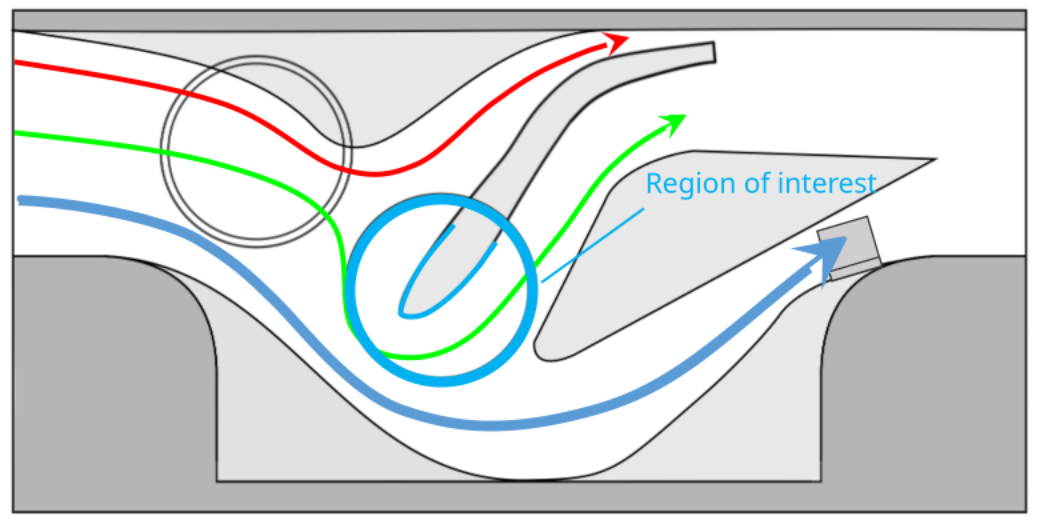
\includegraphics[width=10.1cm,keepaspectratio]{figures/wind_tunnel_with_flow.png}}
  \vspace{.10cm}
  \only<4->{
    \vspace{.10cm}
    \textbf{Tunable inlet Mach number $M_{entry}$}\par
    \small By adjusting the angle of an airfoil aft of the working section.
  }
\end{frame}

\begin{frame}{Aims and research questions}
  \begin{columns}[T]
    \column{.48\textwidth}
    \card{teal}{Aim}{Characterise and quantify the unsteadiness of the shock and separation on the crosswind intake lip.}\\[6pt]
    \card{amber}{Comparison}{Baseline vs.\ \textbf{thinner} vs.\ \textbf{thicker} lip profile.}
    \column{.48\textwidth}
    \textbf{Research questions}
    \begin{enumerate}\setlength\itemsep{.4em}
      \item Where in the $(M_{\mathrm{entry}},\,\mathrm{MFS})$ space does unsteadiness occur?
      \item What are its frequency, amplitude and structure?
      \item How do these change with lip thickness?
      \item \textcolor{amber}{[Add / refine]}
    \end{enumerate}
  \end{columns}
\end{frame}
